%to have line numbers
%\RequirePackage{lineno}
\documentclass[10pt, letterpaper]{article}      
\usepackage[margin=.1cm,font=small,labelfont=bf]{caption}[2007/03/09]
%\usepackage{endnotes}
%\let\footnote=\endnote


\usepackage{setspace}
\usepackage{longtable}                        
\usepackage{anysize}                          
\usepackage{natbib}                           
%\bibpunct{(}{)}{,}{a}{,}{,}                   
\bibpunct{(}{)}{,}{a}{}{,}                   
\usepackage{amsmath}
\usepackage[% draft,
pdftex]{graphicx} %draft is a way to exclude figures                
%\usepackage{epstopdf}
\usepackage{hyperref}                             % For creating hyperlinks in cross references
 
% \usepackage[margins]{trackchanges}

% \note[editor]{The note}
% \annote[editor]{Text to annotate}{The note}
%    \add[editor]{Text to add}
% \remove[editor]{Text to remove}
% \change[editor]{Text to remove}{Text to add}

%TODO make it more standard before submission: \marginsize{2cm}{2cm}{1cm}{1cm}
\marginsize{1cm}{1cm}{.5cm}{.5cm}%{left}{right}{top}{bottom}   
					          % Helps LaTeX put figures where YOU want
 \renewcommand{\topfraction}{1}	                  % 90% of page top can be a float
 \renewcommand{\bottomfraction}{1}	          % 90% of page bottom can be a float
 \renewcommand{\textfraction}{0.0}	          % only 10% of page must to be text

 \usepackage{float}                               %latex will not complain to include float after float

\usepackage[table]{xcolor}                        %for table shading
\definecolor{gray90}{gray}{0.90}
\definecolor{orange}{RGB}{255,128,0}

\renewcommand\arraystretch{.9}                    %for spacing of arrays like tabular

%-------------------- my commands -----------------------------------------
\newenvironment{ig}[1]{
\begin{center}
 %\includegraphics[height=5.0in]{#1} 
 \includegraphics[height=3.3in]{#1} 
\end{center}}

 \newcommand{\cc}[1]{
\hspace{-.13in}$\bullet$\marginpar{\begin{spacing}{.6}\begin{footnotesize}\color{blue}{#1}\end{footnotesize}\end{spacing}}
\hspace{-.13in} }

%-------------------- END my commands -----------------------------------------



%-------------------- extra options -----------------------------------------

\usepackage{pdfpages} %load after xcolor, like at the end ideally i guess and
                      %turn off epstopdf


%%%%%%%%%%%%%
% footnotes %
%%%%%%%%%%%%%

%\long\def\symbolfootnote[#1]#2{\begingroup% %these can be used to make footnote  nonnumeric asterick, dagger etc
%\def\thefootnote{\fnsymbol{footnote}}\footnote[#1]{#2}\endgroup}	%see: http://help-csli.stanford.edu/tex/latex-footnotes.shtml

%%%%%%%%%%%
% spacing %
%%%%%%%%%%%

% \abovecaptionskip: space above caption
% \belowcaptionskip: space below caption
%\oddsidemargin 0cm
%\evensidemargin 0cm

%%%%%%%%%
% style %
%%%%%%%%%

%\pagestyle{myheadings}         % Option to put page headers
                               % Needed \documentclass[a4paper,twoside]{article}
%\markboth{{\small\it Politics and Life Satisfaction }}
%{{\small\it Adam Okulicz-Kozaryn} }

%\headsep 1.5cm
% \pagestyle{empty}			% no page numbers
% \parindent  15.mm			% indent paragraph by this much
% \parskip     2.mm			% space between paragraphs
% \mathindent 20.mm			% indent math equations by this much

%%%%%%%%%%%%%%%%%%
% extra packages %
%%%%%%%%%%%%%%%%%%

\usepackage{datetime}

\usepackage{polski}
\usepackage[utf8]{inputenc}
% \usepackage[latin1]{inputenc}
\usepackage{tikz}
\usetikzlibrary{shapes,arrows,backgrounds}


%\usepackage{color}					% For creating coloured text and background
%\usepackage{float}
\usepackage{subfig}                                     % for combined figures

\renewcommand{\ss}[1]{{\colorbox{blue}{\bf \color{white}{#1}}}}
\newcommand{\ee}[1]{\endnote{\vspace{-.10in}\begin{spacing}{1.0}{\normalsize #1}\end{spacing}\vspace{.20in}}}
\newcommand{\emd}[1]{\ExecuteMetaData[/tmp/tex]{#1}} % grab numbers  from stata

%TODO before submitting comment this out to get 'regular fornt'
\usepackage{sectsty}
\allsectionsfont{\normalfont\sffamily}
\usepackage{sectsty}
\allsectionsfont{\normalfont\sffamily}
\renewcommand\familydefault{\sfdefault}

% \usepackage[margins]{trackchanges} (LM)
\usepackage{rotating}
\usepackage{catchfilebetweentags}

\usepackage{abstract}
\renewcommand{\abstractname}{}    % clear the title
\renewcommand{\absnamepos}{empty} % originally center
%-------------------- END extra options -----------------------------------------
\date{{}\today}
\title{  % remember to have Vistula University!!
Elderly Volunteering and Well-Being in Europe. Revisting Haski (2009) \footnote{This study was funded by grant \# 2016/21/B/HS4/03058 from
  Polish National Science Foundation (Narodowe Centrum Nauki).}
}
\author{
Adam Okulicz-Kozaryn\thanks{EMAIL: adam.okulicz.kozaryn@gmail.com
  \hfill I thank XXX.  All mistakes are mine.} \\
{\small Rutgers - Camden  and Vistula University}
}

\begin{document}

%%\setpagewiselinenumbers
%\modulolinenumbers[1]
%\linenumbers

\bibliographystyle{/home/aok/papers/root/tex/ecta}
\maketitle
\vspace{-.4in}
\begin{center}

\end{center}


\begin{abstract}
\noindent
\end{abstract}
\vspace{.15in} 
\noindent{\sc XXX TODO add to ebib as keyword PAPER-CODE-NAME and tag with ebib keywords 
}
\vspace{.25in} 

\begin{spacing}{1.4} %TODO MAYBE before submission can make it like 2.0
\rowcolors{1}{white}{gray90}

%  instead \ExecuteMetaData[../out/tex]{ginipov} do \emd{ginipov}

% \begin{figure}[H]
%  \includegraphics[height=3in]{../out/gov_res_trust.pdf}\centering\label{gov_res_trust}
% \caption{woo}
% \end{figure}


%TODO !!!! have input here aok_var_des
%%%%%%%%%%%%%%%%%%%%%%%%%%%%%%%%%%%%%%%%%%%%%%%%%%%%%%%%%%%%%%%%%%%%%%%%%%%%%%

Volunteering changes with age not only in its popularity but also in its characteristics. The motives are also presumably different (\citet{wilson12} dodac inne).  From a  economic perspective one may distinguish demand for volunteering that is created by unmet demand for public goods and services and supply of volunteering that depends on how  a person allocate her or his time to unpaid activities to improve her utility \citet{ziemek06}. Economic reasoning  suggests that volunteering should be related to unsatisfactory level of supply of public good and services  that are not delivered by either the market or the government. This implies that unpaid work at the form of volunteering should be more popular in less developed countries where markets are inefficient and quality of goverment is low. However, this prediction is false and volunteering is rather positively  related to the degree of economic development (\citet{Oecd15},Figure 5.1. Participation rates in formal volunteering). Participation rates in formal volunteering range from 57.3\% in Norway to 17.7\% in Czechia. If concentrate on people aged 50 and over in Europe variation in the rates is even larger. It ranges from 37.9\% in the Netherlands to as little as 3.2\% in Poland (\citet{Oecd15}) \footnote{Fig 5.8 Participation rates in formal volunteering among people aged 50 and over in European countries, data are based on the Survey of Health, Ageing and Retirement in Europe (SHARE), wave 4(2015)} \\ 

Higher rates of volunteering in  highly developed countries stres a considerable role of supply factors and the role of public policy in overcoming the barriers to volunteering such as transport difficulties, lack of information, perceptions of volunteering and lack of variety in the opportunities. In the times of rising he problem of ageing volunteering among elderly can play important role in susteining well-being of elderly. Volunteering is beneficial for society (LIT: \citet{Oecd15}, \cite{prouteau06}, ... ). Often it is treated as a productive activity (\citet{hank09}). But it also benefits volunteers. \citet{jenkinson2013volunteering} surveyed forty experimental and cohort studies comparing the physical and mental health outcomes and mortality of a volunteering group to a non-volunteering group and they found that volunteering had favourable effects on depression, life satisfaction, wellbeing but not on physical health. Positive association between vounteering and subjective health was reported in many studies (e.g. \citet{borgonovi08}, (\cite{anderson14}, \cite{li06}, \cite{VanWilligen00}, Japonka,  \citet{detollenaere17}). \\

Quality of life  of elderly has become a major social issue since they are most likely to experience negative events. The assessment of elderly QoL faces is particularly challenging. In response to this a measure of QoL for individuals aged 65 to 75, the so-called CASP-19, based on the needs-satisfaction theory (Maslow, 1943; Doyal and Gough, 1991 has been proposed. This scale includes 19 Likert-type items reflecting four different dimensions of QoL: Control, Autonomy, Self-realization, and Pleasure. A shorter version with 12 items, the so-called CASP-12, was proposed and tested in (Wiggins et al., 2008). A 12-item version of the CASP used in the Survey of Health, Ageing and Retirement in Europe (SHARE) differs from the one suggested in Wiggins(2008). A SPAIN paper supports a multidimensional model for the CASP–12 composed by three factors and it concludes has potential to be used as a multidimensional tool to assess QoL in older people. \\

There is a common agreement in the literature on positive effects on volunteering - those active in such activity report better health and higher scores for subjective well-being (\citet{haski09}, \citet{morrow2003}, \citep{thoits03}, \citep{whillans2016}). \citep{meier08} showed that volunteering led to increased life satisfaction in a longitudinal study in Germany. That is why one also should expect positive relation between volunteering and qulity of life. It is suprising, at least for us, that a question about importance of volunteering (how strong is the volunteering effect on QoL) is asked so rarely. \citet{haski09} is an exceptional example of a data driven study in which that issue was discussed. The study was based on data collected in 2005 and 2006 in the first wave of Survey of Health, Ageing and Retirement in Europe (SHARE). The paper includes an extensive discussion of variations in volunteering rates according to main socio-economic variables as age, gender and employment status among people aged 50 or more in 12 Western and Southern European countries. It finds positive relation between volunteering and physical and psychological well-being and that volunteering rates differes according to country  with the highest rates in Northern Europe and the lowest rates in Southern Europe.  But the puzziling part of the paper is on a relation between volunteering on one side and health and quality of life on the other side. For example, it was found that \textit{"in countries which encourage volunteerism and where volunteering is a social norm, such as in the Northern European countries, the relation of volunteering and wellbeing was rather small. At the same in countries where voulnteering was not so popular  a correlation between volunteering and three indicators of well-being (health, depression, and chances for longer life) were rather strong."}. This was unexpected result. \\

This paper extends the study by \citet{haski09} in a few directions. Firstly, we use data collected in 2015 in the sixth wave of the SHARE survey what allows us to add some Central and Eastern European countries (CEE) into the analysis. The CEE conutries were not previously analyzed since they were not included in the first wave of the survey.  \citep{casiday08} noted that the majority of the papers their review covered were based on data from the United States. Remarkable different life experiences of people from Western Europe and those from Central Europe make new insights into volunteering of population of 50+ possible.  Secondly, in the first wave of the SHARE survey volunteering was identified through a question on activities conducted during last 4 weeks before the interview. As we show in the paper this made the rates of volunteering to be signicantly different to the rates published by the OECD. Starting from the wave 4 of the SHARE the data are based on activities conducted during 12 months preceding the interview. This change has made the volunteering rates in the SHARE more like the statistics from other sources.  Third, association between volunteering and health or life satisfaction is measured in the paper by the Kendall tau coefficient while \citet{haski09} used the Pearson correlations. We also test statistical significance of differences in the correlations coefficients between countries what was not done in the mentioned paper.  Since differences in the correlation coefficients are often quite small it is not obvious if a given difference is really meaningfull. Also, we use different measures of life satisfaction (quality of life) and health to ones used in the reference paper. Finally, we apply a multilevel regresion analysis to control for possible confounders.  \\

Following \citet{haski09} we expect that impact from volunteering on well-being differs among countries and its strength depends on popularity of volunteering. We expect that reation to be negative or convex (inverted U). It means that in countries with the high rates volunteering effect on well-being is lower than in countries with the middle rate. It is not obvious however how important  volunteering might be in countries where it is not popular. Our results can have important practical consequences. Population aging in Europe asks for new policy tools that may be used to keep elderly wellbeing on decent levels. Volunteerism may be an interesting option for elderly and should be considered as a labor supply tool for productive ageing. 
 


\section{Data}

\textbf{About SHARE} \\
We use from the 2015 Survey of Health, Ageing and Retirement in Europe (SHARE). The dataset provides wide range of information on the socio-economic status, health, and family relationships of people in age 50 or more in XY European countries. The wave 6 used in the research is based on XXXXX interviews (CAPI) in 12 countries that were included in the wave 1 (Austria, Belgium, Denmark, France, Germany, Greece, Israel, Italy, Spain, Sweden, Switzerland, and The Netherlands) and 9 countries that entered the survey later on (Czech Republic, Poland, Ireland, Luxembur, Hungary, Portugal, Slovenija, Estonia and Croatia). Over 68 000 elderly  participated in the survey. SHARE applies a concept of ex-ante harmonisation: there is one common generic questionnaire that is translated into the national languages using an internet based translation tool and processed automatically in a common CAPI instrument. \\

\textbf{Sampling} \\
Probability samples were drawn in each participating country. Due to different institutional conditions a uniform sampling design was impossible. For example, a simple random selection of
households, from the central population register was used in in Denmark, while complex multistage design was applied in Greece. The weighted average household response rate was
XX\%, and ranged from XX\% in CC to 74\% in CC. 


\textbf{volunteering} \\
Volunteering differently influences life satisfaction over life course. Willigen (2000) notices that "...elderly experience greater positive changes in their perceived health than did younger adult volunteer".

Volunteering is identified solely on a basis of respondent's declaration about activities conducting in last 12 months. The question was phrased: "Have you done any of these activities in the last month: Done voluntary or charity work." The variable was recoded into a binary variable with the value one for those indicating that activity. Volunteering considered in the study does not include a help given to close family members. This understanding of the volunteering is consistent with the UN definition \footnote{United Nations Volunteers Programme: Preparatory Committee for the Special Session of the General Assembly on the implementation of the outcome of the world summit for social development and further initiatives. Volunteering and social development. A/AC.253/16/Add.7. United Nations; 2000.}. However, one needs to remember that our volunteering measure is not free of possibility of being condaminated by a measurement error. 

Another widely accepted feature of formal volunteerism is that, it takes place within a formal organisational structure, is self-governing, is not profit distributing (?) and is independent of government (Salamon and Sokolowski 2001). Another way of defining voluteering is "informal" volunteering conducted outside of the structures of a voluntary organisation such as providing unpaid help to a friend or neighbour. Informal volunteering includes activities that are very heterogeneous. We are aware that informal and formal volunteering may have very different impact on individuals well being. In the study we include only formal volunteering. Informal is identified in separate question (check to be sure)

\textbf{Quality of life, life satisfaction, CASP} \\
A measure of life satisfaction use in the paper differs from the one applied in Haski(2009). We use the CASP-12 index described in \cite{hyde03}. The CASP-12 is a shorter version of the CASP-19, a measure of quality of life (QoL) in older ages. The CASP-19 draws upon the “Theory of Human Need” and has four dimensions: Control, Autonomy, Self-realization and Pleasure \citep{borrat15}.\\

In the SHARE survey a quality of life is W przypadku badania SHARE ogólne oceny jakości życia respondentów zbierane są przy wykorzystaniu dwóch podejść. Z jednej strony respondenci pytani są o subiektywną ocenę satysfakcji z życia na skali od 0 do 10, a z drugiej odzwierciedlenie oceny jakości życia opiera się o 12 pytań z tzw. zestawu CASP, specjalnie opracowanego na potrzeby badania jakości życia osób we wczesnym okresie starości (w załączniku 1.1 do niniejszego rozdziału znajduje się pełna treść pytań z zestawu CASP). Choć zaletą tego pierwszego podejścia jest przejrzystość i prostota ocen, to wyniki otrzymywane przy wykorzystaniu tego drugiego w mniejszym stopniu narażone są na arbitralność ocen i są mniej zależne od zmiennych czynników silnie wpływających na ogólną ocenę satysfakcji, takich jak nastrój czy pora roku (White, 2007). 
Badanie jakości życia w formie zestawu pytań CASP-12 obecne jest w SHARE od pierwszej edycji projektu. W ramach CASP jakość życia oceniana jest w zależności od poziomu realizacji potrzeb w dziedzinach istotnych dla pozytywnego doświadczania starszego wieku (Hyde i in., 2003): możliwości wpływania na swoje otoczenie (Control), samodzielnego podejmowania decyzji (Autonomy), samorealizacji (Self-realization) i czerpania przyjemności w życiu (Pleasure).  Opierając się o wcześniejsze prace (np. Laslett, 1996) w literaturze wskazuje się, że po odejściu z aktywnego życia zawodowego na emeryturę zwiększa się osobista niezależność i pojawiają nowe możliwości aktywnego udziału w życiu społecznym, podążania za własnymi pragnieniami i rozwijania zainteresowań. 

Tworząc miarę CASP jej autorzy opierali się o teorię potrzeb Maslowa (1968) zakładającą, że ludziom nie zależy wyłącznie na prostym zaspokojeniu potrzeb podstawowych i przetrwaniu, ale konsekwentnie dążą oni do spełnienia potrzeb wyższych, jak szczęście czy poczucie własnej wartości. Rozważania Maslowa autorzy CASP zestawili z poglądem przedstawionym w artykule Doyala i Gougha (1991), iż pierwszeństwo potrzeb fizjologicznych nad społecznymi może być zależne od okoliczności, jako przykład podając osoby starsze oszczędzające na ogrzewaniu, żeby kupić świąteczne prezenty dla wnuków. Z Maslowa autorzy adaptują jeszcze jeden istotny pogląd – iż ludzie współdzielą uniwersalny zestaw potrzeb, co przekłada się na mierzalność poziomu zaspokojenia potrzeb oraz możliwość porównywania tego poziomu dla różnych osób. 



\textbf{health} \\
We use similar measure of subjective health to the one used in Haski(2009). This is the self-perceived health variable with the respondents that range from "very bad" to "very good". Subjective health is also higer in more developed countries. In this case people from Southern European countries repored on average highher levels than those from Eastern Europe. The lowes mean values were found for Poland, Estonia, Croatia, Slovenia, Czech Rep. and in Portugal.

\textbf{Sample selection due to age and health status }\\

\section{Results}

\subsection*{Volunteering rates for elderly in Europe}

The way how a question on volunteering was formulated in the SHARE had significant impact on levels of the rates. The table below compares the rates from Haski (2009) and the rates calculated using the wave 6 with the rates reported in OECD(2016).

%\begin{figure}[H]
% \includegraphics[height=3in]{oecd_oecdShare16.pdf}
% \centering
% \label{fig:volshares}
%\caption{Volunteering shares among 50+}
%\end{figure}
%%% TABLE

\begin{spacing}{.9}
	 \input{OECDSHARE.tex}
      \label{OECDSHARE} 
\end{spacing}
%%%% END: TABLE

The rates in the wave 6 are much more like the rates published by the OECD than the rates from the wave 1. Changes in the question made volunteering rates in the SHARE more similar to those published by the OECD using the Gallup data. The rates from the wave 6 exceeds those from the wave 1 except Sweden (18\% vs. 15\%).  For example, for Switzerland the rate is almost 30\%, while previously it was 15\%. For Germany the rate changed from 17\% to almost 25\%. The rates in countries that did not particpated in the wave 1 are low - Poland 3.43\%, Czech Republic 8.87\%, Estonia 8.75\%, Portugal 9.55\%, Slovenia 12.15\%. Only for Luxemburg the rate is high - 24.75\%. Similar to previous studies , the results show significant country variation in volunteering rates. The pattern found in the SHARE data is well know in literature - the highest rates are in Northern and Western Europe:  Denmark (31.4\%), Switzerland (29.5\%) and Belgium (26.6\%), and the lowest rates are in Eastern and Southern Europe: Poland (3.4\%), Spain (6.3\%), Greece (7.0\%) and Czech Republic (8.9\% [Lit.]. It is intresting that he scores in formerly centrally-planned economies such as Poland, Czech Rep., Estonia or Croatia are higher than in Southern Europe. We may speculate that an economic progress in Eastern and Central Europe that have been observed since the collapse of the communism is an one possible explanation. The range of the values from above 30\% to as little above 3\% suggest other explanations than simple differences in demographic structure.   Despite that levels published by the OECD and those calculated from the SHARE data are different the geographical pattern in which low values are in Southern and Central Europe and high values re in  Western and Northern Europe is consistent. \footnote{Results for Sweden \textit{are somehow couterintuitive and difficut to interpret. Lower values in the wave 6 than in the wave 1 suggest that less elderly were egaged in volunteering in 2015 than in 2006. ??? }} \\



\subsection*{Kendall-tau and significance test - volunteering vs. subjective health and casp}

\footnote{based on PEARSON'S VERSUS SPEARMAN'S AND KENDALL'S CORRELATION COEFFICIENTS FOR CONTINUOUS DATA, Nian Shong Chok, 2008}

We analyse relation between popularity of volunteering and its impact on wellbeing using Kendall's correlation coefficients. We decided to use the Kendall's measure since it is usually suggested for non-normally distributed data and that the Pearson correlation coefficient is appropriate only for interval data. On the other hand, the Kendall's correlation coefficients can be used for either ordinal or interval data. According to Khamis  Kendall's tau is more appropriate if at least one variable is ordinal one \footnote{Khamis H. Measures of Association: How to Choose? Journal of Diagnostic Medical Sonography. 2008;24:155-162.}. Kendall's tau is less sensitive to outliers and is often preferred due to its simplicity and ease of interpretation. The Kendall'a tau(b) correlation coefficients for association between volunteering and subjective health or subjective wellbeing  are presented below together with the countries rates of volunteering.


\begin{figure}[H]
\centering
\caption{Tau b correlations} 
\label{fig:taub}
\begin{minipage}{1\linewidth}
\subfloat[Subjective health]{\includegraphics[height=2.7in]{Kendall_h.pdf}}\quad
\subfloat[CASP]{\includegraphics[height=2.7in]{Kendall_casp.pdf}}~\\
{\footnotesize Notes: }~\\
{\footnotesize Source: Own calculations based on SHARE Wave 6.}
\end{minipage}
\end{figure} 

%
%\begin{figure}[H]
% \includegraphics[height=3in]{Kendall_h.pdf}
% \centering
% \label{fig:tauH}
%\caption{tau subjective health}
%\end{figure}


In all countries volunteering and subjective health are positively associated. The highest association was denoted in Luxemburg (the Kendall's correlation of 18.0\%) and the lowest in Sweden (1.7\%). In Western and Northern Europe the associations are stronger than in Southern and Central Europe but the differences between some countries from both groups are rather small. This suggests that increasing popularity of volunteering in Poland, Czech Republic, Italy or Spain will not necessarily be associated with significant change in subjective health of volunteers. The significance tests for differences between tau(b) are given in the Appendix. According to these tests the difference between Germany and Poland with the corresponding rates of volunteering of 23.8\% and 3.4\% is not statisitically significant. The same we conclude for difference between Germany and Czech Republic where the rate of volunteering is 8.9\%. Other pairs with similar associations between volunteering and health and large differences in popularity of volunteering are: Denmark and Poland, Denmark and Czech Republic, Denmark and Spain, Denmark and Portugal.  \\


As it was expected association between volunteering and CASP  is positive. The Kendall's correlation coefficients range from 15.4\% (Isreal) to 3.3\% (Sweden).  The nonlinear, inverted U-shape relation, is easily seen. For example, the coefficients for Germany and Belgium are on a similar level as those in Slovenia, Portugal and Spain despite about 10 pp. difference between the rates of volunteering between for example Germany and Slovenia. Also, the differences between Poland and Czech Republic on an one side and Italy and Estonia on another are highly significant (pvalues about 1\%). These significances come together with small differences in the volunteering rates. Our findings do not allow us to reject the hypothesis about nonlinearity in the relation between popularity of volunteering and its effect on wellbeing. \\

The puzzeling outcome of \citet{haski09} was unexpected pattern of correlations between  popularity of volunteering and wellbeing.  The more recent data from the SHARE survey with more countries, a different measure of volunteering and a different measure of association confirms that finding - weak volunteering effect is observed among low rate countries (Czech Republic, Greece, Portugal, Slovenia) and among high rate countries (Denmark, Switzeralnd, Belgium, Luxemburg, Germany). Somewhere between the impact is the strongest. \\

Neither the Pearson's correlation nor the Kendall's correlation coefficient  do not control for confounding variables. They just describe unconditional relation betweem volunteering and well-being. To account for the role of possible confounding variables we run a regression analysis.   

\subsection*{Volunteering and casp, health (unconditional means)}

% Casp v volunteering
So fat we have compared simple uncondtional means for volunteers and non-volunteers what once againg reveals a division into West$-$Nord and Central$-$South Europe. Volunteers report on average higher values of casp. Differences between the conditional scores are smaller among  high income coutries. The absolute difference for Denmark  is 0.9, for Switzerland 1.1 and for Greece 2.1, for Portugal 2.4 and for Isreal 2.9. The highest absolute difference of 3.8 is for Poland and the second to the highest if for Estonia (3.6). The pattern for relative differences is very similar with high heterogenity among countries where the rates are low and much lower heterogenity in countries where the rates are large \footnote{This may be a statistical fact due to larger number of observations that causes variance to be smaller}. 
Unconditional means do not show previously noticed non-linearity. Here, we rather see negative linear realtion with large heterogenity among countries with low volunteering rates.

Volunteers give on average better answer about subjective health. Comparing conditional mean scores reveals different pattern to the one discussed for casp. There is weaker relation between popularity of volunteering in a country and its impact on subjective health. 


\begin{figure}[H]
\centering
\caption{Unconditional means} 
\label{fig:vol_casp}
\begin{minipage}{1\linewidth}
\subfloat[CASP]{\includegraphics[height=2.7in]{rel_casp.pdf}}\quad
\subfloat[CASP]{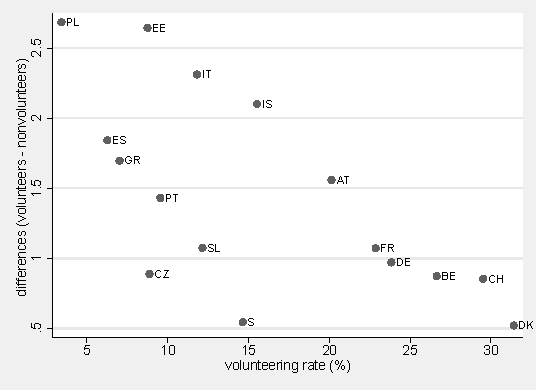
\includegraphics[height=2.7in]{abs_casp.pdf}} \quad
\subfloat[Health]{\includegraphics[height=2.7in]{rel_health.pdf}}\quad
\subfloat[Health]{\includegraphics[height=2.7in]{abs_health.pdf}} ~\\
{\footnotesize Notes: }~\\
{\footnotesize Source: Own calculations based on SHARE Wave 6.}
\end{minipage}
\end{figure} 

\subsection*{Volunteering and casp (conditional means - simple regression analysis)}

The estmiated model for $casp_{i,c}$ with i standing for a person and c for a country was:

 \begin{eqnarray}
	casp_{i,c}= \beta_{0}+ \beta_{1}*v_{i,c} + \beta_{2}*r_{c}*v_{i,c}+\beta_{3}*r^{2}_{c}*v_{i,c}+\gamma*Z_{i,c} + \epsilon_{i,c}
 \end{eqnarray}
 
where $v_{i,c}$ is a binary variable equal to 1 if a person i from a country c is engaged in  volunteering, $r_{c}$ is a country volunteering rate calculted from the wave 6 of the SHARE survey and a matrix $Z_{i,c}$ includes controls : age,gender, education measured in years and a country average gdp per capita expressed in purchasing power parity in years X-Y. In the model we pool the data for all countries and we assume that individuals within a country share unobserved characteristics. In order to account for the within-country correlation across observations we apply cluster-robust  standard errors with clusters being the countries. To control for the differences in endowments between volunteers and non-volunteers we additionally apply the mean decomposition:

 \begin{eqnarray}
	\bar{\hat{casp_{c}}}(1)-\bar{\hat{casp_{c}}}(0)= (\hat{\beta_{1}}+\hat{\beta_{2}}*r_{c}+\hat{\beta_{3}}*r^{2}_{c})+\hat{\gamma}*(\bar{Z}_{c}(1)-\bar{Z}_{c}(0))
 \end{eqnarray}
       
with $\hat{casp_{i,c}(1)}$ being a predicted average wellbeing for a volunteer and $\hat{casp_{i,c}(0)}$ is a predicted average wellbeing for a non-volunteer.  The first term gives an impact of volunteering as function of its popularity in a country. The second term, an endowment effect, controls for differences in covariates between volunteers and non volunteers. As we see in the model differences in wellbeing are explained by different levels of volunteering ($ r_{c}$) but also by differences in endowments allocated into volunteering ($\bar{Z}_{c}(1)$) and into non-volunteering ($\bar{Z}_{c}(0)$). However, thought differences in characteristcs allocated to both sectors may matter among countries they are valued exactly in the same way ($\gamma$). In the model we may fully decompose the total mean $\bar{casp}$ since $\bar{casp} = \bar{\hat{casp}}$ but the observed and predicted means on country levels are not equal. \\ 

One can fit a separate model to each country’s dataset if she or he wants to obtaine a model with decomosable differences on a country level: 

 \begin{eqnarray}
	casp_{i,c}= \beta_{0c}+ \beta_{1c}*v_{i,c} + \gamma_{c}*Z_{i,c} + \epsilon_{i,c}
 \end{eqnarray}


Here, any country effect is absorbed into the country-specific intercept term in each country’s regression model. For each country we get separate coefficient for an effect of volunteering.  No restrictions are assumed on the variance of the error terms for each country. The mean decomposition in this case is:

 \begin{eqnarray}
	\bar{\hat{casp_{c}}}(1)-\bar{\hat{casp_{c}}}(0)= \hat{\beta_{0c}}+\hat{\gamma_{c}}*(\bar{Z}_{c}(1)-\bar{Z}_{c}(0))
 \end{eqnarray}

With this specification $\bar{casp_{c}} = \bar{\hat{casp_c}}$ what allows for full decomposition of the difference in conditional means of casp. 


The full estimation results are given in the Appendix. For pooled model we gest a concave relation between the rate of volunteering and wellbeing suggesting decreasing marginal impact from volunteering to wellbeing (Fig.3 (a)). Panel b shows the decomposition of the means for that model. Panel c presents unconditinal means while panel d shows their decompositions into endowments effect and volunteering effec using teh country-specific models. 

\begin{figure}[H]
\centering
\caption{Volunteering and wellbeing (OLS)} 
\label{fig:casp_ols}
\begin{minipage}{1\linewidth}
\subfloat[Predicted wellbeing]{\includegraphics[height=2.7in]{ols_margins.pdf}}\quad
\subfloat[Decomposition (Pooling)]{\includegraphics[height=2.7in]{ols_fit.pdf}}\quad
\subfloat[Differences in means]{\includegraphics[height=2.7in]{abs_dcasp.pdf}} \quad
\subfloat[Decomposition (Separate models)]{\includegraphics[height=2.7in]{ols_fitcry.pdf}}~\\
{\footnotesize Notes: }~\\
{\footnotesize Source: Own calculations based on SHARE Wave 6.}
\end{minipage}
\end{figure} 
   
Interpretion ? (What can we say ? Results are very different. Pooling suggests that volunteers are better off becouse they have better characteristics. It is not voluteering make them more satisfied but rather they are volunteers becouse they are more satified. Volunteering is more important when it is not very popular. When the volunteering is very popular it is possible for volunteering to lower wellbeing. Why ? It may be that you are socially forced to do that and you do not enjoy it. Separate models give different impression. Country differences are much more evident. VOlunteering is more important than it was suggested by the previous model. Better people select into volunteering but also, despite their previleged characteristics, they get extra wellbeing from volunteering. )//



Another way how the relation between volunteering and wellbeing can be discussed here is by using the multilevel liner regression modelling since we may define two levels in the data  - the individuals and the countries. By allowing for a random intercept for each country in the model we allow for different values for individial casp within a country after controlling for gender, age and other control variables. At the same time we allow for a variation in averages between countries.  Below the results of two models are summarised. The first model assumed the varying intercept, while the seocond is based on the formulation to be known as the growth model. The first model is: \\


 \begin{eqnarray}
	casp_{i,j}\sim N(\beta_{0}+ c_{j} +  \beta_{1,j} * vol_{i,j}+\gamma*Z_{i,j},\sigma^{2}_{y}) \\	
	c_{j} \sim N(\gamma_{c},\sigma^{2}_{c}) \\
	\beta_{1,j} \sim N(\gamma_{r}*r^{2}_{j},\sigma^{2}_{r})
 \end{eqnarray}


%Full regression results are given in the Appendix. Using the same decomposition we may compare results from OLS estimation of linear regression model with the MLM estimation: 
%
%
%\begin{figure}[H]
%\centering
%\caption{Effect of volunteering on wellbeing (OLS v MLM) } 
%\label{fig:casp_mlm}
%\begin{minipage}{1\linewidth}
%\subfloat[OLS]{\includegraphics[height=2.7in]{ols_fit.pdf}}\quad
%\subfloat[MLM]{\includegraphics[height=2.7in]{mlm_fit.pdf}} ~\\
%{\footnotesize Notes: }~\\
%{\footnotesize Source: Own calculations based on SHARE Wave 6.}
%\end{minipage}
%\end{figure}   
%
%Results are much different ... 

The quadratic growth model with a random effect for countries is an extension of regression model (citep{•}):
 
\begin{eqnarray}
	casp_{i,j}\sim N(\beta_{0}+ c_{j} +  \beta_{1}*v_{i,c} + \beta_{2}*r_{c}*v_{i,c}+\beta_{3}*r^{2}_{c}*v_{i,c}+\gamma*Z_{i,c} + \epsilon_{i,c}
 \end{eqnarray}
 
 The model allows for $\beta_{0}+ c_{j}$ instead of assuming fixed value of $\beta_{0}$.   

\begin{figure}[H]
\centering
\caption{Volunteering and wellbeing (Multilevel Linear Model)} 
\label{fig:casp_ols}
\begin{minipage}{1\linewidth}
\subfloat[Varying intercept model]{\includegraphics[height=2.7in]{mlmQ_fit0.pdf}}\quad
\subfloat[Quadratic growth model]{\includegraphics[height=2.7in]{mlmQ_fit1.pdf}} ~\\
{\footnotesize Notes: }~\\
{\footnotesize Source: Own calculations based on SHARE Wave 6.}
\end{minipage}
\end{figure}  
 
Interpretation ...  
 
\section{Discussion}


The positive consequences of being engaged in volunteering by elderly are well known and commonly accepted. Volunteering is important and it needs to be study in details.  According to OECD estimates the value of unpaid volunteering ranges from X\% of GDP to as much as Y\% (OECD, yyyy).  Demographic changes combined with progress in health care add to increasing time while people are in relatively good health while being on retirement. This creates additional  stock of unused labor among elderly that may be effectively used with benefit for volunteer and other members of a society.  It makes   volunteering of elderly to be potentially important policy tool that may help to keep people in better health when they get older. \\


Casual realtion between volunteering  and health or wellbeing is not obvious. Volunteering may improve the employability of volunteers and it provides engagement in a socially meaningful role  what could positively impact on health and well-being. Volunteering might builts up social networks and gives meaning and purpose in life. (przepisana, zmodyfikowane) //

The question that must be asked is whether popularization of volunteering should be put into social policy agenda. Taking into consideration our results we expect different answers in different countries. It is possible that in some rich and highly developed countries volunteering is so popular and treated as so usuall activity that it adds only marginally to individuals' wellbeing. 

\begin{thebibliography}{87}
\newcommand{\enquote}[1]{``#1''}
\expandafter\ifx\csname natexlab\endcsname\relax\def\natexlab#1{#1}\fi

\bibitem[\protect\citeauthoryear{Anderson, Damianakis, Kr{\"o}ger, Wagner, Dawson, Binns, Bernstein, Caspi, and Cook}{Anderson
  et~al.}{2014}]{anderson14}
\textsc{Anderson, N.~D., T.~Damianakis, E.~Kr{\"o}ger, L.~M. Wagner, D.~R.Dawson, M.~A. Binns, S.~Bernstein, E.~Caspi, and S.~L. Cook} (2014):  \enquote{The benefits associated with volunteering among seniors: a critical  review and recommendations for future research.} \emph{Psychological bulletin}, 140, 1505.


\bibitem[\protect\citeauthoryear{Borgonovi}{Borgonovi}{2008}]{borgonovi08}
\textsc{Borgonovi, F.} (2008): \enquote{Doing well by doing good. The relationship between formal volunteering and self$-$reported health and happiness,} \emph{Social Science and Medicine}, 66,  2321 -- 2334.

\bibitem[\protect\citeauthoryear{Borrat-Besson, Ryser and Gonçalves}{Borrat-Besson et~al.}{2015}]{borrat15}
\textsc{Borrat-Besson, C.,V-A.~Ryser, and J.~Gonçalves} (2015):  \enquote{What impact does it really have?} \emph{An evaluation of the CASP-12 scale used in the Survey of Health, Ageing and Retirement in Europe (SHARE) to measure Quality of Life among people aged 50+}, \emph{FORS Working Papers}, 2015-4


\bibitem[\protect\citeauthoryear{Casiday, Kinsman, Fisher and Bambra}{Casiday et~al.}{2008}]{casiday08}
\textsc{Casiday, R., E.~Kinsman, C.~Fisher and C.~Bambra} (2008):  \enquote{What impact does it really have?} \emph{Report to Volunteering England}, London: Volunteering England.

\bibitem[\protect\citeauthoryear{Detollenaere, Willems, Baert}{Detollenaere et~al.}{2017}]{detollenaere17}
\textsc{Detollenaere, J. and S.~Willems and S.~Baert} (2017): \enquote{Volunteering, income and health,} \emph{PLoS ONE}, 12(3):e0173139,  doi:10.1371/journal.pone.0173139.

\bibitem[\protect\citeauthoryear{Haski-Leventhal}{Haski-Leventhal}{2009}]{haski09}
\textsc{Haski-Leventhal, D.} (2009): \enquote{Elderly volunteering and
  well-being: A cross-European comparison based on SHARE data,} \emph{Voluntas:
  International Journal of Voluntary and Nonprofit Organizations}, 20,
  388--404.
  
  % Potwierdzeni CASP in SHARE
%@article{doi:10.1080/13607863.2017.1292208,
%author = {Gema Pérez-Rojo and Noemy Martín and Cristina Noriega and Javier López},
%title = {Psychometric properties of the CASP-12 in a Spanish older community dwelling sample},
%journal = {Aging \& Mental Health},
%volume = {0},
%number = {0},
%pages = {1-9},
%year  = {2017},
%abstract = {Objective: Current studies have shown that older people's quality of life (QoL) is more associated to individual's sense of happiness and subjective life satisfaction than to objective problems. CASP scale conceptualizes QoL based on a psycho-sociological perspective. Originally, CASP consisted of 19 items (four factors: Control, Autonomy, Self-realization and Pleasure). Later, it was proposed a shorter version (12 items and three factors). The aim of this study was to assess the structure of the CASP-12 SHARE version using confirmatory factor analysis.  
  
\bibitem[\protect\citeauthoryear{Hank and Erlinghagen}{Hank and
  Erlinghagen}{2009}]{hank09}
\textsc{Hank, K. and M.~Erlinghagen} (2009): \enquote{Dynamics of volunteering in older Europeans,} \emph{The Gerontologist}, 50, 170--178.  

\bibitem[\protect\citeauthoryear{Hyde}{Hyde}{2003}]{hyde03}
\textsc{Hyde, M.} (2003): \enquote{A measure of quality of life in early old age: The theory, development and properties of a needs satisfaction model (CASP-19),} \emph{Aging and mental health}, 7(3), 186--194. 


\bibitem[\protect\citeauthoryear{Jenkinson, Dickens, Jones, Thompson-Coon, Taylor, Rogers, Bambra, Lang, and Richards}{Jenkinson et~al.}{2013}]{jenkinson2013volunteering}
\textsc{Jenkinson, C.~E., A.~P. Dickens, K.~Jones, J.~Thompson-Coon, R.~S.Taylor, M.~Rogers, C.~L. Bambra, I.~Lang, and S.~H. Richards} (2013):
  \enquote{Is volunteering a public health intervention? A systematic review and meta-analysis of the health and survival of volunteers,} \emph{BMC public health}, 13, 773.

\bibitem[\protect\citeauthoryear{Li and Ferraro}{Li and Ferraro}{2006}]{li06}
\textsc{Li, Y. and KF.~Ferraro} (2006): \enquote{Volunteering in middle and later life: is health a benefit, barrier or both ?} \emph{Social Forces}, 85, 497--519. 


\bibitem[\protect\citeauthoryear{Meier and Stutzer}{Meier and
  Stutzer}{2008{\natexlab{b}}}]{meier08}
---\hspace{-.1pt}---\hspace{-.1pt}--- (2008{\natexlab{b}}): \enquote{Is volunteering rewarding in itself?} \emph{Economica}, 75, 39--59.

\bibitem[\protect\citeauthoryear{Morrow-Howell, Hinterlong, Rozario and Tang}{Morrow-Howell et~al.}{2003}]{morrow2003}
\textsc{Morrow-Howell, N., J.~Hinterlong, P.~A.Rozario, F.~Tang} (2003):
  \enquote{Effects of Volunteering on the Well-Being of Older Adults,} \emph{The Journals of Gerontology: Series B},58, S137--S145


\bibitem[\protect\citeauthoryear{Oecd}{Oecd}{2015}]{Oecd15}
\textsc{Oecd} (2015): \enquote{How's Life  2015 - Measuring Well-being} \emph{OECD 2015}.
  
 \bibitem[\protect\citeauthoryear{Prouteau and Wolff}{Prouteau and Wolff}{2006}]{prouteau06}
\textsc{Prouteau, L. and ~F-C.Wolff } (2006): \enquote{Does volunteer work pay off in the labor market?,} \emph{Journal of Socio-Economics}, 35, 992--1013.

 \bibitem[\protect\citeauthoryear{Thoits and Hewitt}{Thoits and Hewitt}{2001}]{thoits03}
\textsc{Thoits, P.A. and ~L.N.Hewitt } (2001): \enquote{Volunteer Work and Well-Being,} \emph{Volunteer Work and Well-Being},42, 115--131.


\bibitem[\protect\citeauthoryear{Whillans, Seider, Chen, Dwyer, Novick, Gramign, Mitchell, Savalei, Dickerson and Dunn}{Whillans et~al.}{2016}]{whillans2016}
\textsc{Whillans, A.~V., S.~C. Seider, L.~Chen, R.~J. Dwyer, S.~Novick, K.~J.Gramign, B.~A. Mitchell, V.~Savalei, S.~S.Dickerson and E.~W. Dunn}(2016):
  \enquote{Does volunteering improve well-being?,} \emph{omprehensive Results in Social Psychology}, 1, 35--50.

  
\bibitem[\protect\citeauthoryear{Wilson}{Wilson}{2012}]{wilson12}
\textsc{Wilson, J.} (2012): \enquote{Volunteerism research: A
  review essay,} \emph{Nonprofit and Voluntary Sector Quarterly}, 41, 176--212.

\bibitem[\protect\citeauthoryear{Ziemek}{Ziemek}{2006}]{ziemek06}
\textsc{Ziemek, S.} (2006): \enquote{Economic analysis of volunteers` motivations. A cross$-$country study,} \emph{Journal of Socio$-$Economics}, 35(3), 532--555.


\bibitem[\protect\citeauthoryear{Van Willigen}{Van Willigen}{2000}]{VanWilligen00}
\textsc{Van Willigen, M.} (2000): \enquote{Differential benefits of volunteering across the life course,} \emph{Journal of Gerontology Series B}, 55, 5308--5318.


\end{thebibliography}


\begin{spacing}{.9}

\section{Appendix: additional descriptive statistics}

\begin{figure}[H]
 \includegraphics[height=3in]{oecd_age50p.pdf}
 \centering
% \source{ }
 \label{fig:oecd_50p}
\caption{volunteering shares}
\end{figure}

% Rozkład CASP
\begin{figure}[H]
 \includegraphics[height=3in]{hist_casp.pdf}
 \centering
 \label{fig:hist_casp}
\caption{Distribution of CASP by countries}
\end{figure}

%%%%%%%%%%%%%%%%%%  DESCRIPTIVES %%%%%%%%%%%%%%%%%%%%%%%%%

% Descriptives of CASP condtional on volunteering
\begin{spacing}{.9}
	 % Table generated by Excel2LaTeX from sheet 'Sheet1'
\begin{table}[H]
  \centering
  \caption{Casp conditional on volunteering}
    \begin{tabular}{lcccccccccccc}
          & \multicolumn{3}{p{12.165em}}{p10} & \multicolumn{3}{p{12.165em}}{mean} & \multicolumn{3}{p{12.165em}}{median} & \multicolumn{3}{p{12.165em}}{p90} \\
    volunteering & no    & yes   & total & no    & yes   & total & no    & yes   & total & no    & yes   & total \\
    Denmark & 35.0  & 37.0  & 35.0  & 41.1  & 42.0  & 41.4  & 42.0  & 43.0  & 42.0  & 47.0  & 47.0  & 47.0 \\
    Switzerland & 34.0  & 36.0  & 34.0  & 40.5  & 41.6  & 40.8  & 41.0  & 42.0  & 42.0  & 46.0  & 46.0  & 46.0 \\
    Austria & 32.0  & 36.0  & 32.0  & 39.4  & 41.7  & 39.9  & 40.0  & 42.0  & 41.0  & 46.0  & 47.0  & 46.0 \\
    Luxembourg & 32.0  & 35.0  & 32.0  & 39.4  & 41.1  & 39.8  & 40.0  & 42.0  & 41.0  & 46.0  & 46.0  & 46.0 \\
    Sweden & 33.0  & 34.0  & 33.0  & 39.5  & 40.1  & 39.6  & 40.0  & 41.0  & 40.0  & 45.0  & 46.0  & 45.0 \\
    Germany & 31.0  & 34.0  & 32.0  & 38.8  & 40.5  & 39.2  & 40.0  & 41.0  & 40.0  & 45.0  & 46.0  & 45.0 \\
    Belgium & 29.0  & 32.0  & 30.0  & 37.9  & 39.6  & 38.3  & 39.0  & 40.0  & 39.0  & 45.0  & 46.0  & 45.0 \\
    Slovenia & 30.0  & 34.0  & 30.0  & 38.1  & 40.3  & 38.3  & 39.0  & 41.0  & 39.0  & 45.0  & 46.0  & 45.0 \\
    France & 29.0  & 32.0  & 30.0  & 37.5  & 39.5  & 37.9  & 38.0  & 40.0  & 39.0  & 45.0  & 46.0  & 45.0 \\
    Croatia & 27.0  & 33.0  & 28.0  & 35.9  & 39.1  & 36.1  & 37.0  & 39.0  & 37.0  & 44.0  & 45.5  & 44.0 \\
    Spain & 27.0  & 32.0  & 28.0  & 35.9  & 39.1  & 36.1  & 36.0  & 40.0  & 37.0  & 44.0  & 45.0  & 44.0 \\
    Poland & 27.0  & 33.0  & 27.0  & 35.7  & 39.5  & 35.9  & 36.0  & 40.0  & 36.0  & 45.0  & 45.5  & 45.0 \\
    Czech Republic & 29.0  & 30.0  & 29.0  & 35.5  & 36.7  & 35.6  & 36.0  & 37.0  & 36.0  & 42.0  & 43.0  & 42.0 \\
    Estonia & 27.0  & 32.0  & 27.0  & 35.1  & 38.7  & 35.4  & 35.0  & 39.0  & 36.0  & 43.0  & 45.0  & 44.0 \\
    Italy & 26.0  & 31.0  & 26.0  & 34.5  & 37.8  & 34.9  & 35.0  & 38.0  & 35.0  & 43.0  & 45.0  & 43.0 \\
    Israel & 28.0  & 31.0  & 28.0  & 34.4  & 37.3  & 34.8  & 34.0  & 38.0  & 34.0  & 43.0  & 44.0  & 43.0 \\
    Portugal & 25.0  & 29.0  & 26.0  & 33.1  & 35.5  & 33.4  & 33.0  & 35.0  & 34.0  & 40.0  & 42.0  & 41.0 \\
    Greece & 25.0  & 26.0  & 25.0  & 31.7  & 33.8  & 31.8  & 32.0  & 34.0  & 32.0  & 39.0  & 41.0  & 39.0 \\
    Total & 28.0  & 33.0  & 29.0  & 36.6  & 39.8  & 37.1  & 37.0  & 41.0  & 38.0  & 45.0  & 46.0  & 45.0 \\
    \end{tabular}%
  \label{tab:addlabel}%
\end{table}%

      \label{CASP}
\end{spacing}
%%%% END: TABLE

% Descriptives of subjective health condtional on volunteering

\begin{spacing}{.9}
	 % Table generated by Excel2LaTeX from sheet 'Sheet1'
\begin{table}[H]
  \centering
  \caption{Subjective health conditionally on volunteering}
    \begin{tabular}{ccccccc}
          & \multicolumn{3}{c}{poor} & \multicolumn{3}{c}{at leas very good} \\
    volunteering & no    & yes   & total & no    & yes   & total \\
    Switzerland & 0.039 & 0.012 & 0.031 & 0.364 & 0.475 & 0.396 \\
    Denmark & 0.055 & 0.031 & 0.048 & 0.533 & 0.640 & 0.566 \\
    Sweden & 0.049 & 0.039 & 0.048 & 0.398 & 0.420 & 0.401 \\
    Belgium & 0.060 & 0.020 & 0.049 & 0.256 & 0.360 & 0.283 \\
    Austria & 0.070 & 0.021 & 0.060 & 0.289 & 0.455 & 0.322 \\
    Luxembourg & 0.076 & 0.035 & 0.066 & 0.256 & 0.406 & 0.293 \\
    Greece & 0.067 & 0.068 & 0.067 & 0.344 & 0.395 & 0.348 \\
    Italy & 0.080 & 0.032 & 0.074 & 0.222 & 0.267 & 0.228 \\
    Germany & 0.094 & 0.028 & 0.078 & 0.175 & 0.266 & 0.197 \\
    France & 0.116 & 0.045 & 0.100 & 0.192 & 0.288 & 0.214 \\
    Israel & 0.105 & 0.071 & 0.100 & 0.355 & 0.411 & 0.364 \\
    Spain & 0.111 & 0.038 & 0.106 & 0.210 & 0.287 & 0.215 \\
    Czech Republic & 0.133 & 0.063 & 0.127 & 0.162 & 0.277 & 0.173 \\
    Slovenia & 0.144 & 0.053 & 0.132 & 0.145 & 0.215 & 0.153 \\
    Croatia & 0.188 & 0.036 & 0.181 & 0.251 & 0.360 & 0.256 \\
    Portugal & 0.195 & 0.127 & 0.188 & 0.077 & 0.120 & 0.081 \\
    Estonia & 0.201 & 0.067 & 0.189 & 0.053 & 0.162 & 0.063 \\
    Poland & 0.210 & 0.050 & 0.204 & 0.083 & 0.117 & 0.085 \\
    Total & 0.109 & 0.037 & 0.097 & 0.235 & 0.366 & 0.256 \\
    \end{tabular}%
  \label{tab:addlabel}%
\end{table}%

      \label{sphus}
\end{spacing}
%%%% END: TABLE


%%%%%%%%%%%%%%%%%%  TAU %%%%%%%%%%%%%%%%%%%%%%%%%

%%% TABLE
\begin{spacing}{.9}
	 % Table generated by Excel2LaTeX from sheet 'Health'
\begin{table}[H]
  \centering
  \caption{Volunteering and health (taub): pvalues}
    \begin{tabular}{lrrrrrrrrrrrrr}
          & \multicolumn{1}{c}{AT} & \multicolumn{1}{c}{FR} & \multicolumn{1}{c}{BE} & \multicolumn{1}{c}{CH} & \multicolumn{1}{c}{DE} & \multicolumn{1}{c}{DK} & \multicolumn{1}{c}{CZ} & \multicolumn{1}{c}{IT} & \multicolumn{1}{c}{SE} & \multicolumn{1}{c}{PL} & \multicolumn{1}{c}{IS} & \multicolumn{1}{c}{GR} & \multicolumn{1}{c}{S} \\
          & \multicolumn{1}{c}{0.201} & \multicolumn{1}{c}{0.229} & \multicolumn{1}{c}{0.266} & \multicolumn{1}{c}{0.295} & \multicolumn{1}{c}{0.239} & \multicolumn{1}{c}{0.314} & \multicolumn{1}{c}{0.089} & \multicolumn{1}{c}{0.118} & \multicolumn{1}{c}{0.147} & \multicolumn{1}{c}{0.034} & \multicolumn{1}{c}{0.155} & \multicolumn{1}{c}{0.07} & \multicolumn{1}{c}{0.063} \\
          & \multicolumn{1}{c}{-0.162} & \multicolumn{1}{c}{-0.125} & \multicolumn{1}{c}{-0.123} & \multicolumn{1}{c}{-0.121} & \multicolumn{1}{c}{-0.112} & \multicolumn{1}{c}{-0.099} & \multicolumn{1}{c}{-0.085} & \multicolumn{1}{c}{-0.082} & \multicolumn{1}{c}{-0.081} & \multicolumn{1}{c}{-0.073} & \multicolumn{1}{c}{-0.04} & \multicolumn{1}{c}{-0.021} & \multicolumn{1}{c}{-0.017} \\
    AT    &       &       &       &       &       &       &       &       &       &       &       &       &  \\
    FR    & 0.079 &       &       &       &       &       &       &       &       &       &       &       &  \\
    BE    & 0.045 & 0.904 &       &       &       &       &       &       &       &       &       &       &  \\
    CH    & 0.071 & 0.845 & 0.92  &       &       &       &       &       &       &       &       &       &  \\
    DE    & 0.015 & 0.497 & 0.539 & 0.675 &       &       &       &       &       &       &       &       &  \\
    DK    & 0.003 & 0.202 & 0.208 & 0.33  & 0.528 &       &       &       &       &       &       &       &  \\
    CZ    & 0     & 0.041 & 0.036 & 0.098 & 0.168 & 0.49  &       &       &       &       &       &       &  \\
    IT    & 0     & 0.022 & 0.017 & 0.064 & 0.108 & 0.38  & 0.864 &       &       &       &       &       &  \\
    SE    & 0     & 0.017 & 0.013 & 0.053 & 0.09  & 0.341 & 0.811 & 0.946 &       &       &       &       &  \\
    PL    & 0     & 0.029 & 0.027 & 0.061 & 0.101 & 0.283 & 0.601 & 0.688 & 0.723 &       &       &       &  \\
    IS    & 0     & 0.001 & 0.001 & 0.003 & 0.005 & 0.025 & 0.076 & 0.091 & 0.098 & 0.258 &       &       &  \\
    GR    & 0     & 0     & 0     & 0     & 0     & 0     & 0.001 & 0.001 & 0.001 & 0.027 & 0.446 &       &  \\
    S     & 0     & 0     & 0     & 0     & 0     & 0     & 0.001 & 0.001 & 0.001 & 0.022 & 0.383 & 0.864 &  \\
    \end{tabular}%
  \label{tab:addlabel}%
\end{table}%

      \label{tauH} 
\end{spacing}
%%%% END: TABLE

%%% TABLE
\begin{spacing}{.9}
	 % Table generated by Excel2LaTeX from sheet 'Lilfe Sat.'
\begin{table}[H]
  \centering
  \caption{Add caption}
    \begin{tabular}{lrrrrrrrrrrrrr}
          & \multicolumn{1}{p{4.785em}}{IS} & \multicolumn{1}{c}{AT} & \multicolumn{1}{c}{IT} & \multicolumn{1}{c}{FR} & \multicolumn{1}{c}{DE} & \multicolumn{1}{c}{SE} & \multicolumn{1}{c}{BE} & \multicolumn{1}{c}{PL} & \multicolumn{1}{c}{CH} & \multicolumn{1}{c}{GR} & \multicolumn{1}{c}{DK} & \multicolumn{1}{c}{CZ} & \multicolumn{1}{c}{S} \\
          & \multicolumn{1}{c}{0.155} & \multicolumn{1}{c}{0.201} & \multicolumn{1}{c}{0.118} & \multicolumn{1}{c}{0.229} & \multicolumn{1}{c}{0.239} & \multicolumn{1}{c}{0.147} & \multicolumn{1}{c}{0.266} & \multicolumn{1}{c}{0.03} & \multicolumn{1}{c}{0.295} & \multicolumn{1}{c}{0.07} & \multicolumn{1}{c}{0.314} & \multicolumn{1}{c}{0.089} & \multicolumn{1}{c}{0.063} \\
          & \multicolumn{1}{c}{0.154} & \multicolumn{1}{c}{0.141} & \multicolumn{1}{c}{0.144} & \multicolumn{1}{c}{0.123} & \multicolumn{1}{c}{0.109} & \multicolumn{1}{c}{0.103} & \multicolumn{1}{c}{0.101} & \multicolumn{1}{c}{0.09} & \multicolumn{1}{c}{0.086} & \multicolumn{1}{c}{0.082} & \multicolumn{1}{c}{0.064} & \multicolumn{1}{c}{0.053} & \multicolumn{1}{c}{0.033} \\
    IS    & 0.584 &       &       &       &       &       &       &       &       &       &       &       &  \\
    IT    & 0.641 & 0.879 &       &       &       &       &       &       &       &       &       &       &  \\
    FR    & 0.19  & 0.362 & 0.237 &       &       &       &       &       &       &       &       &       &  \\
    DE    & 0.05  & 0.089 & 0.036 & 0.434 &       &       &       &       &       &       &       &       &  \\
    SE    & 0.021 & 0.034 & 0.009 & 0.24  & 0.711 &       &       &       &       &       &       &       &  \\
    BE    & 0.018 & 0.026 & 0.006 & 0.203 & 0.636 & 0.914 &       &       &       &       &       &       &  \\
    PL    & 0.015 & 0.025 & 0.01  & 0.136 & 0.38  & 0.538 & 0.593 &       &       &       &       &       &  \\
    CH    & 0.006 & 0.009 & 0.003 & 0.067 & 0.238 & 0.362 & 0.41  & 0.84  &       &       &       &       &  \\
    GR    & 0.002 & 0.001 & 0     & 0.022 & 0.117 & 0.201 & 0.241 & 0.71  & 0.875 &       &       &       &  \\
    DK    & 0     & 0     & 0     & 0.002 & 0.015 & 0.027 & 0.035 & 0.25  & 0.309 & 0.316 &       &       &  \\
    CZ    & 0     & 0     & 0     & 0     & 0.001 & 0.002 & 0.003 & 0.09  & 0.105 & 0.087 & 0.546 &       &  \\
    S     & 0     & 0     & 0     & 0     & 0     & 0     & 0     & 0.01  & 0.012 & 0.006 & 0.109 & 0.281 &  \\
    \end{tabular}%
  \label{tab:addlabel}%
\end{table}%

      \label{tauLS} 
\end{spacing}
%%%% END: TABLE

%%%%%%%%%%%%%%%%%%  LINEAR REGRESSION (OLS) %%%%%%%%%%%%%%%%%%%%%%%%%

%% TABLE : klopoty z formatowaniem 
\begin{spacing}{.9}
\begin{table}[H]
\centering 
\caption{CASP vs. volunteering and gdp per capita (Linear model, OLS)}  
\begin{scriptsize} 
	 {
\def\sym#1{\ifmmode^{#1}\else\(^{#1}\)\fi}
\begin{tabular}{l*{4}{c}}
\hline\hline
                    &\multicolumn{1}{c}{(1)}&\multicolumn{1}{c}{(2)}&\multicolumn{1}{c}{(3)}&\multicolumn{1}{c}{(4)}\\
                    &\multicolumn{1}{c}{casp}&\multicolumn{1}{c}{casp}&\multicolumn{1}{c}{casp}&\multicolumn{1}{c}{casp}\\
\hline
vol                 &        1.10***&        0.75*  &        0.50   &               \\
ageint              &       -0.01   &       -0.01   &       -0.01   &       -0.01   \\
Male or female      &       -0.01   &       -0.00   &       -0.00   &       -0.00   \\
yedu\_av             &        0.12*  &        0.12*  &        0.11*  &        0.11*  \\
1b.sphus            &        0.00   &        0.00   &        0.00   &        0.00   \\
2.sphus             &       -1.34***&       -1.34***&       -1.34***&       -1.34***\\
3.sphus             &       -2.37***&       -2.36***&       -2.37***&       -2.37***\\
4.sphus             &       -4.08***&       -4.07***&       -4.08***&       -4.08***\\
5.sphus             &       -6.21***&       -6.21***&       -6.21***&       -6.21***\\
averageGDP          &        0.10+  &        0.10+  &        0.10+  &        0.10+  \\
avGDP2              &       -0.00   &       -0.00   &       -0.00   &       -0.00   \\
v1volrate           &               &        1.73   &        4.95   &               \\
v1volrate2          &               &               &       -8.39   &               \\
0b.vol              &               &               &               &        0.00   \\
1.vol               &               &               &               &        0.50   \\
volrate0            &               &               &               &        4.95   \\
0b.vol#co.volrate0  &               &               &               &        0.00   \\
1o.vol#co.volrate0  &               &               &               &        0.00   \\
c.volrate0#c.volrate0&               &               &               &       -8.39   \\
0b.vol#co.volrate0#co.volrate0&               &               &               &        0.00   \\
1o.vol#co.volrate0#co.volrate0&               &               &               &        0.00   \\
constant            &       33.20***&       33.32***&       33.33***&       33.33***\\
\hline
N                   &       46485   &       46485   &       46485   &       46485   \\
\hline\hline
\end{tabular}
}

      \label{regOLS} 
\end{scriptsize}
\end{table}
\end{spacing}
%%% END: TABLE

Chcę dodać descriptives (means), ale nie umiem :( Próbowałem z outreg2..., sum. Tex się nie kompiluje do pdf.



%%%%%%%%%%%%%%%%%%  MLM %%%%%%%%%%%%%%%%%%%%%%%%%

%%% TABLE
\begin{spacing}{.9}
\begin{table}[H]
\centering 
\caption{CASP vs. volunteering and gdp per capita (Multilevel Linear Model)}  
\begin{scriptsize} 
	 {
\def\sym#1{\ifmmode^{#1}\else\(^{#1}\)\fi}
\begin{tabular}{l*{1}{c}}
\hline\hline
            &\multicolumn{1}{c}{casp}\\
\hline
volunteering&        0.90***\\
age: 60-70  &        0.42***\\
age: 71+    &       -0.08   \\
female      &       -0.08+  \\
edu         &        0.06***\\
health:excellent&        6.82***\\
health:very good&        5.74***\\
health:good &        4.35***\\
health:fair &        2.37***\\
income      &        0.00***\\
gdp         &        0.25***\\
gdp sq      &       -0.00** \\
BE          &       -1.74***\\
DK          &       -0.12   \\
FR          &       -1.54***\\
DE          &       -0.81** \\
S           &       -1.24***\\
CH          &        1.70   \\
LU          &       21.96*  \\
GR          &       -6.87***\\
IS          &       -4.48***\\
PT          &       -3.02***\\
IT          &       -3.83***\\
ES          &       -2.47***\\
CZ          &       -3.10***\\
PL          &        1.38** \\
constant    &       22.27***\\
sd(vol)     &        0.23***\\
sd(Residual)&        4.51***\\
\hline
N           &       45764   \\
\hline\hline
\end{tabular}
}

      \label{regB} 
\end{scriptsize}
\end{table}
\end{spacing}
%%%% END: TABLE

\section{Statistical Appendix}

1. Kendall tau b \\
2. Multilevel Linear Regresion Model

\end{spacing}
\end{spacing}
\end{document}
